\section{How do GANs work?}

We have now seen several other generative models and explained that GANs do not
work in the same way that they do. But how do GANs themselves work?

\subsection{The GAN framework}

The basic idea of GANs is to set up a game between two players.
One of them is called the \newterm{generator}.
The generator creates samples that are intended to come from the
same distribution as the training data.
The other player is the \newterm{discriminator}.
The discriminator examines samples to determine whether they are real
or fake.
The discriminator learns using traditional supervised learning techniques,
dividing inputs into two classes (real or fake).
The generator is trained to fool the discriminator.
We can think of the generator as being like a counterfeiter, trying to
make fake money, and the discriminator as being like police, trying to
allow legitimate money and catch counterfeit money.
To succeed in this game, the counterfeiter must learn to make money that
is indistinguishable from genuine money, and the generator network must
learn to create samples that are drawn from the same distribution as the
training data.
The process is illustrated in \figref{fig:framework}.

\begin{figure}
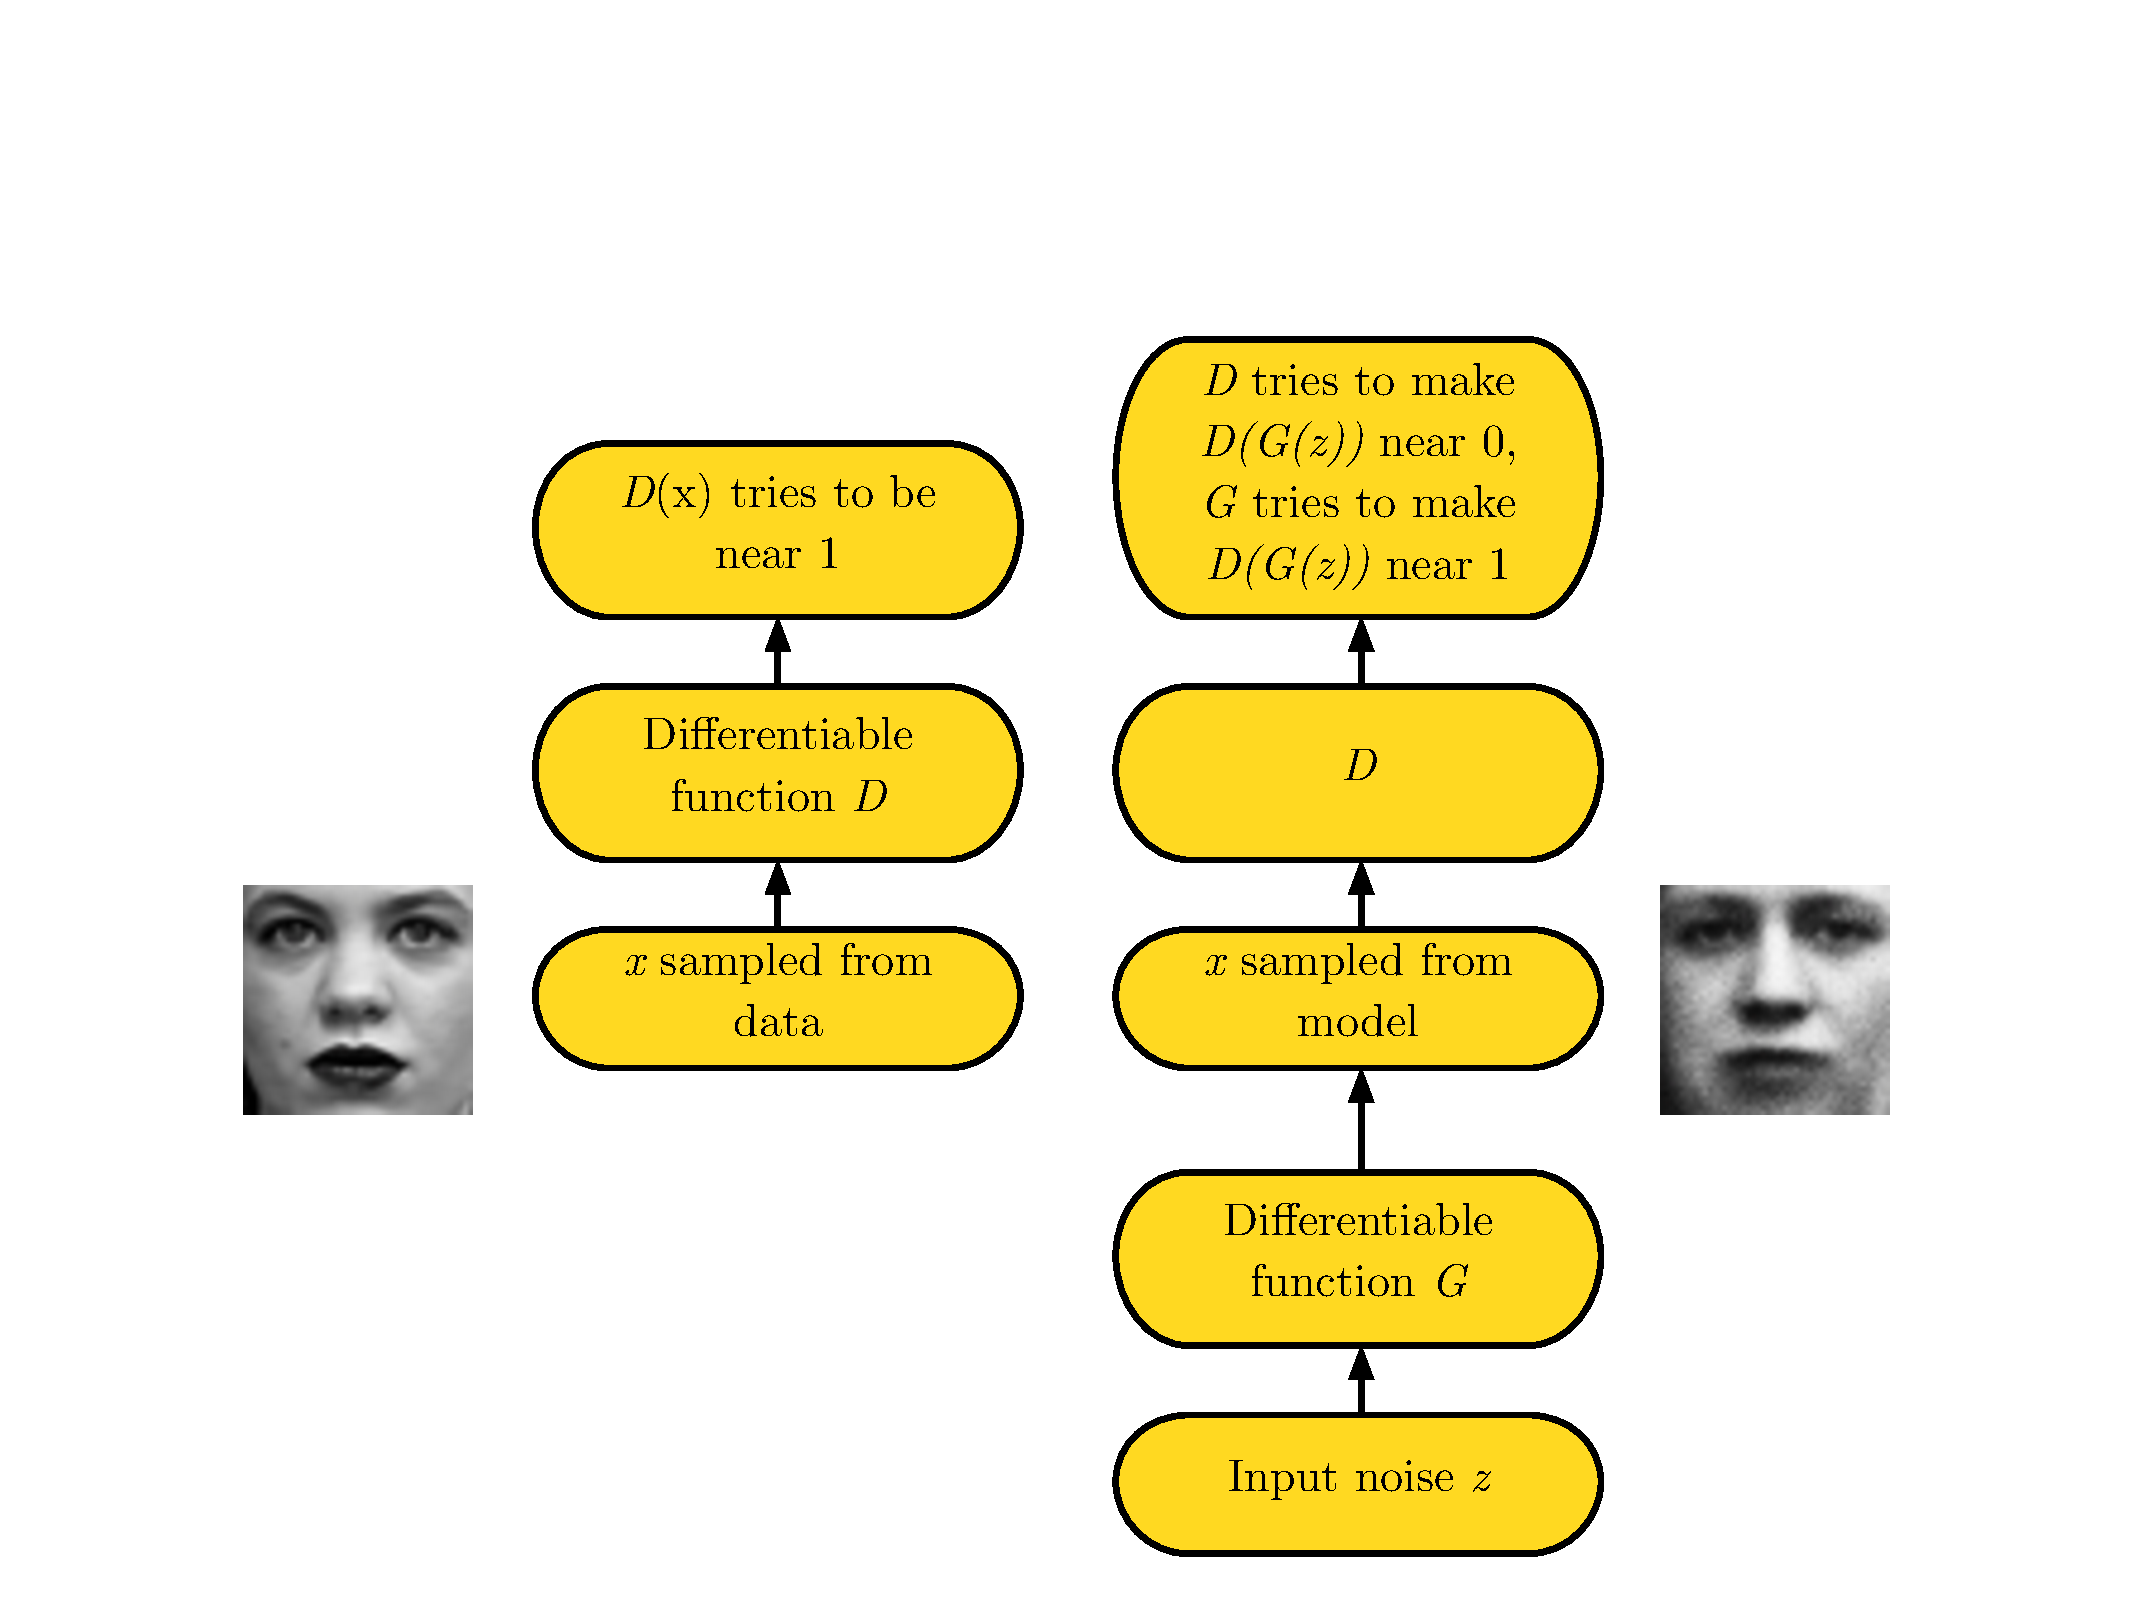
\includegraphics[width=\textwidth]{framework}
\caption{The GAN framework pits two adversaries against each other in a game.
Each player is represented by a differentiable function controlled by a set
of parameters.
Typically these functions are implemented as deep neural networks.
The game plays out in two scenarios.
In one scenario, training examples $\vx$ are randomly sampled from the training
set and used as input for the first player, the discriminator, represented
by the function $D$. The goal of the discriminator is to output the probability
that its input is real rather than fake, under the assumption that half of the
inputs it is ever shown are real and half are fake.
In this first scenario, the goal of the discriminator is for $D(\vx)$ to be
near 1.
In the second scenario, inputs $\vz$ to the generator are randomly sampled from
the model's prior over the latent variables.
The discriminator then receives input $G(\vz)$, a fake sample created by the
generator.
In this scenario, both players participate. The discriminator strives to make
$D(G(z))$ approach 0 while the generative strives to make the same quantity
approach 1.
If both models have sufficient capacity, then the Nash equilibrium of this game
corresponds to the $G(\vz)$ being drawn from the same distribution as the training
data, and $D(\vx) = \frac{1}{2}$ for all $\vx$.
}
\label{fig:framework}
\end{figure}

Formally, GANs are a structured probabilistic model (see chapter 16 of
\citet{Goodfellow-et-al-2016} for an introduction to structured probabilistic
models) containing latent variables $\vz$ and observed variables $\vx$.
The graph structure is shown in \figref{fig:graph}.

The two players in the game are represented by two functions, each of which
is differentiable both with respect to its inputs and with respect to its
parameters.
The discriminator is a function $D$ that takes $\vx$ as input and uses
$\vtheta^{(D)}$ as parameters.
The generator is defined by a function $G$ that takes $\vz$ as input and
uses $\vtheta^{(G)}$ as parameters.

Both players have cost functions that are defined in terms of both players'
parameters.
The discriminator wishes to minimize $J^{(D)}\left( \vtheta^{(D)}, \vtheta^{(G)} \right)$
and must do so while controlling only $\vtheta^{(D)}$.
The generator wishes to minimize $J^{(G)}\left( \vtheta^{(D)}, \vtheta^{(G)} \right)$
and must do so while controlling only $\vtheta^{(G)}$.
Because each player's cost depends on the other player's parameters, but each player
cannot control the other player's parameters, this scenario is most
straightforward to describe as a game rather than as an optimization problem.
The solution to an optimization problem is a (local) minimum, a point in parameter space
where all neighboring points have greater or equal cost.
The solution to a game is a Nash equilibrium.
Here, we use the terminology of local differential Nash equilibria \citep{ratliff2013characterization}.
In this context, a Nash equilibrium is a tuple $(\vtheta^{(D)}, \vtheta^{(G)} )$
that is a local minimum of $J^{(D)}$ with respect to $\vtheta^{(D)}$ and a local
minimum of $J^{(G)}$ with respect to $\vtheta^{(G)}$.

\paragraph{The generator}
The generator is simply a differentiable function $G$.
When $\vz$ is sampled from some simple prior distribution,
$G(\vz)$ yields a sample of $\vx$ drawn from $\pmodel$.
Typically, a deep neural network is used to represent $G$.
Note that the inputs to the function $G$ do not need to correspond
to inputs to the first layer of the deep neural net; inputs may
be provided at any point throughout the network.
For example, we can partition $\vz$ into two vectors $\vz^{(1)}$
and $\vz^{(2)}$, then feed $\vz^{(1)}$ as input to the first layer
of the neural net and add $\vz^{(2)}$ to the last layer of the neural
net. If $\vz^{(2)}$ is Gaussian, this makes $\vx$ conditionally Gaussian
given $\vz^{(1)}$.
Another popular strategy is to apply additive or multiplicative noise to
hidden layers or concatenate noise to hidden layers of the neural net.
Overall, we see that there are very few restrictions on the design of
the generator net.
If we want $\pmodel$ to have full support on $\vx$ space we need the dimension
of $\vz$ to be at least as large as the dimension of $\vx$, and $G$ must be
differentiable, but those are the only requirements.
In particular, note that any model that can be trained with the nonlinear
ICA approach can be a GAN generator network.
The relationship with variational autoencoders is more complicated;
the GAN framework can train some models that the VAE framework cannot and vice
versa, but the two frameworks also have a large intersection.
The most salient difference is that, if relying on standard backprop,
VAEs cannot have discrete variables at the input to the generator,
while GANs cannot have discrete variables at the output of the generator.

\paragraph{The training process}
The training process consists of simultaneous SGD.
On each step, two minibatches are sampled: a minibatch of $\vx$ values from
the dataset and a minibatch of $\vz$ values drawn from the model's prior over
latent variables.
Then two gradient steps are made simultaneously:
one updating $\vtheta^{(D)}$ to reduce $J^{(D)}$
and one updating $\vtheta^{(G)}$ to reduce $J^{(G)}$.
In both cases, it is possible to use the gradient-based optimization algorithm
of your choice.
Adam \citep{kingma2014adam} is usually a good choice.
Many authors recommend running more steps of one player than the other, but
as of late 2016, the author's opinion is that the protocol that works the best
in practice is simultaneous gradient descent, with one step for each player.


\begin{figure}
  \centering
  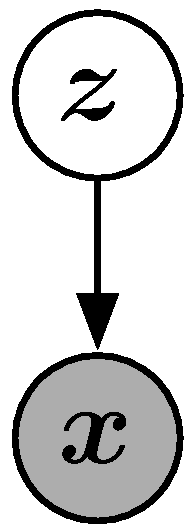
\includegraphics{graph}
  \caption{The graphical model structure of GANs, which is also shared with
    VAEs, sparse coding, etc.
    It is directed graphical model where every latent variable influences
    every observed variable.
    Some GAN variants remove some of these connections.
  }
  \label{fig:graph}
\end{figure}

\subsection{Cost functions}

Several different cost functions may be used within the GANs framework.

\subsubsection{The discriminator's cost, $J^{(D)}$}

All of the different games designed for GANs so far use the same cost for the
discriminator, $J^{(D)}$. They differ only in terms of the cost used for the
generator, $J^{(G)}$.

The cost used for the discriminator is:
\begin{equation}
  J^{(D)}(\vtheta^{(D)}, \vtheta^{(G)}) = -\frac{1}{2} \E_{\vx \sim \pdata} \log D(\vx) - \frac{1}{2} \E_{\vz} \log \left(1 - D\left( G(z)\right) \right).
  \label{eq:discriminator_cost}
\end{equation}

This is just the standard cross-entropy cost that is minimized when training a standard binary classifier
with a sigmoid output.
The only difference is that the classifier is trained on two minibatches of data; one coming from the
dataset, where the label is $1$ for all examples, and one coming from the generator, where the label
is $0$ for all examples.

All versions of the GAN game encourage the discriminator to minimize \eqref{eq:discriminator_cost}.
In all cases, the discriminator has the same optimal strategy.
The reader is now encouraged to complete the exercise in \secref{sec:opt_d} and review its solution
given in \secref{sec:opt_d_soln}. This exercise shows how to derive the optimal discriminator strategy
and discusses the importance of the form of this solution.

We see that by training the discriminator, we are able to obtain an estimate of the ratio
\[
  \frac{\pdata(\vx)}{\pmodel(\vx)}
\]
at every point $\vx$.
Estimating this ratio enables us to compute a wide variety of divergences and their gradients.
This is the key approximation technique that sets GANs apart from variational autoencoders
and Boltzmann machines.
Other deep generative models make approximations based on lower bounds or Markov chains;
GANs make approximations based on using supervised learning to estimate a ratio of two densities.
The GAN approximation is subject to the failures of supervised learning: overfitting and underfitting.
In principle, with perfect optimization and enough training data, these failures can be overcome.
Other models make other approximations that have other failures.

Because the GAN framework can naturally be analyzed with the tools of game theory,
we call GANs ``adversarial.'' But we can also think of them as cooperative, in
the sense that the discriminator estimates this ratio of densities and then freely
shares this information with the generator.
From this point of view, the discriminator is more like a teacher instructing the
generator in how to improve than an adversary.
So far, this cooperative view has not led to any particular change in the development
of the mathematics.

\subsubsection{Minimax}
\label{sec:minimax}

So far we have specified the cost function for only the discriminator.
A complete specification of the game requires that we specify a cost function also
for the generator.

The simplest version of the game is a \newterm{zero-sum game}, in which the sum of all player's
costs is always zero.
In this version of the game,
\begin{equation}
J^{(G)} = - J^{(D)}.
\label{eq:minimax}
\end{equation}

Because $J^{(G)}$ is tied directly to $J^{(D)}$, we can summarize the entire game with a
\newterm{value function} specifying the discriminator's payoff:
\[ V\left(\vtheta^{(D)}, \vtheta^{(G)} \right) = - J^{(D)} \left(\vtheta^{(D)}, \vtheta^{(G)} \right).\]

Zero-sum games are also called \newterm{minimax} games because their solution involves minimization
in an outer loop and maximization in an inner loop:
\[ \vtheta^{(G)*} = \argmin_{\vtheta^{(G)}} \max_{\vtheta^{(D)}} V\left(\vtheta^{(D)}, \vtheta^{(G)} \right) . \]

The minimax game is mostly of interest because it is easily amenable to theoretical analysis.
\citet{Goodfellow-et-al-NIPS2014-small} used this variant of the GAN game to show that learning in
this game resembles minimizing the Jensen-Shannon divergence between the data and the model distribution,
and that the game converges to its equilibrium if both players' policies can be updated directly in
function space.
In practice, the players are represented with deep neural nets and updates are made in parameter space,
so these results, which depend on convexity, do not apply.

\subsubsection{Heuristic, non-saturating game}
\label{sec:heuristic}

The cost used for the generator in the minimax game (\eqref{eq:minimax}) is useful for theoretical analysis,
but does not perform especially well in practice.

Minimizing the cross-entropy between a target class and a classifier's predicted distribution
is highly effective because the cost never saturates when the classifier has the wrong output.
The cost does eventually saturate, approaching zero, but only when the classifier has already
chosen the correct class.

In the minimax game, the discriminator minimizes a cross-entropy, but the generator maximizes
the same cross-entropy.
This is unfortunate for the generator, because when the discriminator successfully rejects
generator samples with high confidence, the generator's gradient vanishes.

To solve this problem, one approach is to continue to use cross-entropy minimization for the
generator.
Instead of flipping the sign on the discriminator's cost to obtain a cost for the generator,
we flip the target used to construct the cross-entropy cost.
The cost for the generator then becomes:
\[
  J^{(G)} = -\frac{1}{2} \E_\vz \log D(G(\vz))
\]

In the minimax game, the generator minimizes the log-probability of the discriminator being correct.
In this game, the generator maximizes the log-probability of the discriminator being mistaken.

This version of the game is heuristically motivated, rather than being motivated by a theoretical
concern.
The sole motivation for this version of the game is to ensure that each player has a strong
gradient when that player is ``losing'' the game.

In this version of the game, the game is no longer zero-sum, and cannot be described with a single
value function.

\subsubsection{Maximum likelihood game}
\label{sec:mle_gan}

We might like to be able to do maximum likelihood learning with GANs, which would mean minimizing
the KL divergence between the data and the model, as in \eqref{eq:kl}.
Indeed, in \secref{sec:tree}, we said that GANs could optionally implement maximum likelihood,
for the purpose of simplifying their comparison to other models.

There are a variety of methods of approximating \eqref{eq:kl} within the GAN
framework.
\citet{Goodfellow-ICLR2015} showed that using
\[ J^{(G)} = -\frac{1}{2} \E_z \exp\left( \sigma^{-1} \left( D(G(\vz)) \right) \right), \]
  where $\sigma$ is the logistic sigmoid function, is equivalent to minimizing \eqref{eq:kl},
  under the assumption that the discriminator is optimal.
  This equivalence holds in expectation; in practice, both stochastic gradient descent on the KL
  divergence and the GAN training procedure will have some variance around the true expected
  gradient due to the use of sampling (of $\vx$ for maximum likelihood and $\vz$ for GANs)
  to construct the estimated gradient.
  The demonstration of this equivalence is an exercise (\secref{sec:mle_exercise}
  with the solution in \secref{sec:mle_soln}).


  Other methods of approximating maximum likelihood within the GANs framework are possible.
  See for example \citet{nowozin2016f}.
  
 

  \subsubsection{Is the choice of divergence a distinguishing feature of GANs?}
  \label{sec:which_divergence}

  As part of our investigation of how GANs work, we might wonder exactly what it is
  that makes them work well for generating samples.

  Previously, many people (including the author) believed that GANs produced sharp,
  realistic samples because they minimize the Jensen-Shannon divergence while
  VAEs produce blurry samples because they minimize the KL divergence between the
  data and the model.

  The KL divergence is not symmetric; minimizing $\KL(\pdata \Vert \pmodel)$
  is different from minimizing $\KL(\pmodel \Vert \pdata)$.
  Maximum likelihood estimation performs the former; minimizing the Jensen-Shannon
  divergence is somewhat more similar to the latter.
  As shown in \figref{fig:kl}, the latter might be expected to yield better samples
  because a model trained with this divergence would prefer
  to generate samples that come only from modes in the training distribution
  even if that means ignoring some modes, rather than
  including all modes but generating some samples that do not come 
  from any training set mode.

  \begin{figure}
    \centering
    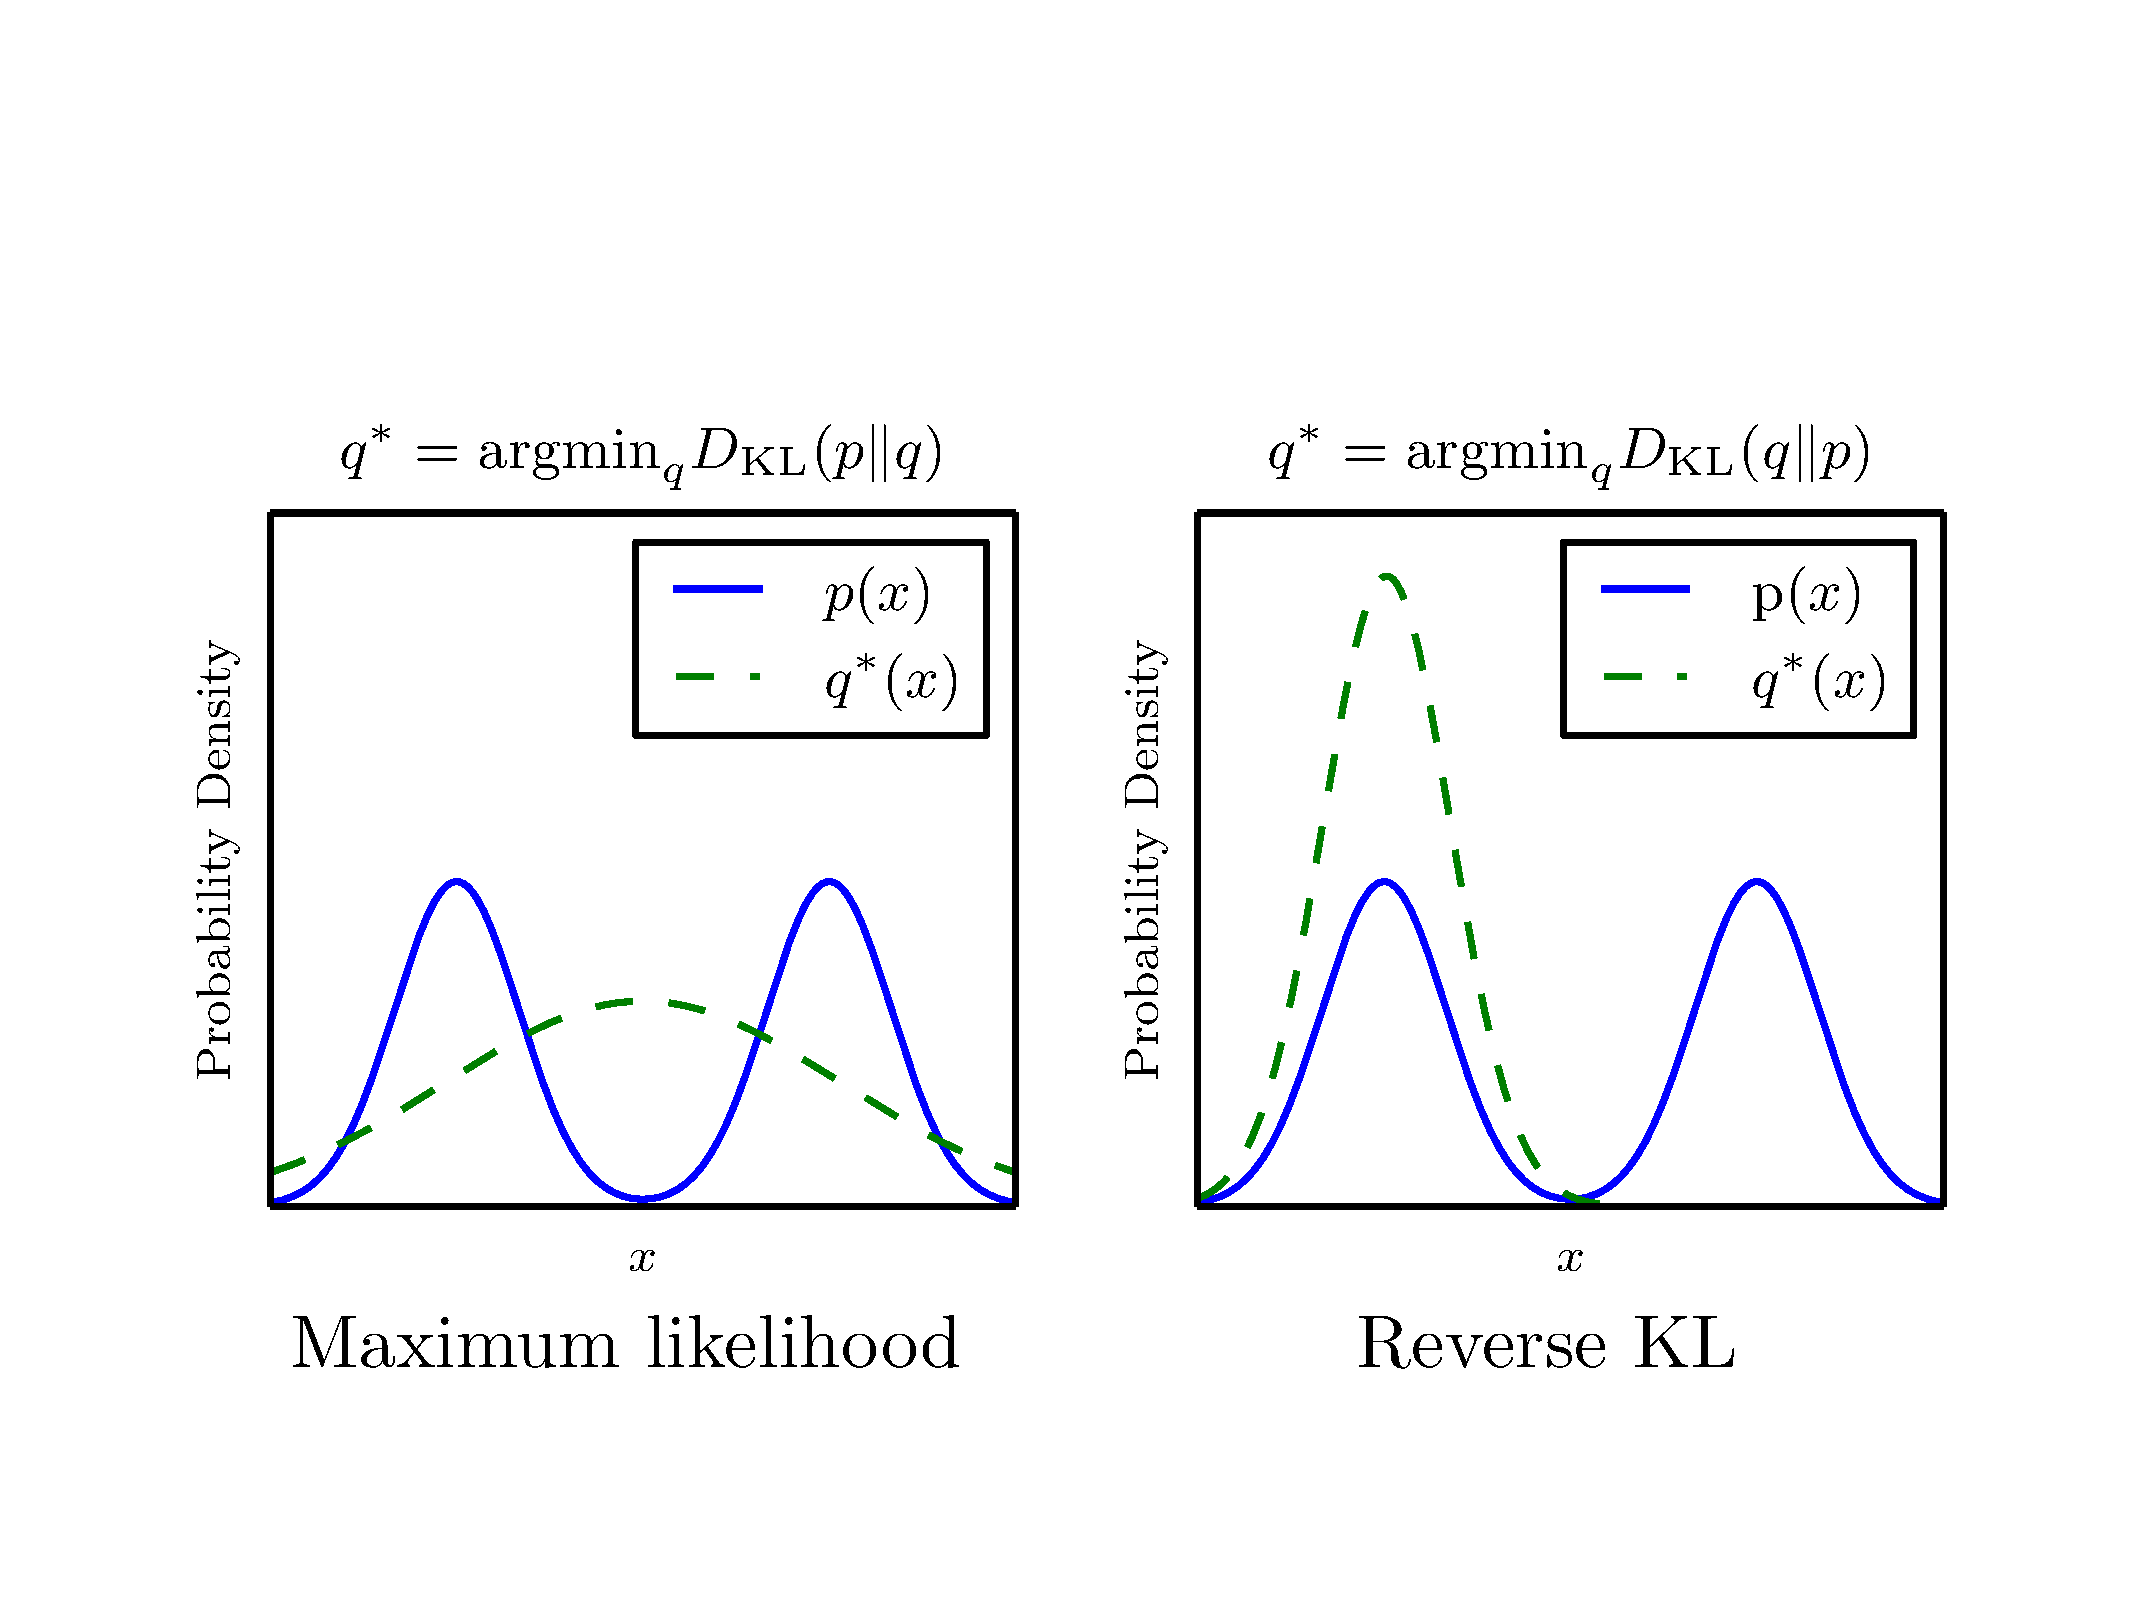
\includegraphics[width=\figwidth]{kl}
    \caption{
The two directions of the KL divergence are not equivalent.
The differences are most obvious when the model has too little
capacity to fit the data distribution.
Here we show an example of a distribution over one-dimensional
data $x$.
In this example, we use a mixture of two Gaussians as the data
distribution, and a single Gaussian as the model family.
Because a single Gaussian cannot capture the true data distribution,
the choice of divergence determines the tradeoff that the model makes.
On the left, we use the maximum likelihood criterion.
The model chooses to average out the two modes, so that it places high
probability on both of them.
On the right, we use the reverse order of the arguments to the KL
divergence, and the model chooses to capture only one of the two modes.
It could also have chosen the other mode; the two are both local minima
of the reverse KL divergence.
We can think of $\KL( \pdata \Vert \pmodel )$ as preferring to place
high probability everywhere that the data occurs,
and $\KL( \pmodel \Vert \pdata )$ as preferrring to place low probability
wherever the data does not occur.
From this point of view, one might expect
$\KL( \pmodel \Vert \pdata )$
to yield more visually pleasing samples,
because the model will not choose to generate unusual samples lying
between modes of the data generating distribution.
    }
    \label{fig:kl}
  \end{figure}

Some newer evidence suggests that the use of the Jensen-Shannon divergence does
not explain why GANs make sharper samples:
\begin{itemize}
  \item It is now possible to train GANs using maximum likelihood, as described in
    \secref{sec:mle_gan}.
    These models still generate sharp samples, and still select a small number of modes.
    See \figref{fig:fgan}.
  \item
    GANs often choose to generate from very few modes; fewer than the limitation
    imposed by the model capacity.
    The reverse KL prefers to generate from {\em as many modes of the data distribution as the model is able to};
    it does not prefer fewer modes in general.
    This suggests that the mode collapse is driven by a factor other than the choice 
    of divergence.
\end{itemize}

\begin{figure}
\centering
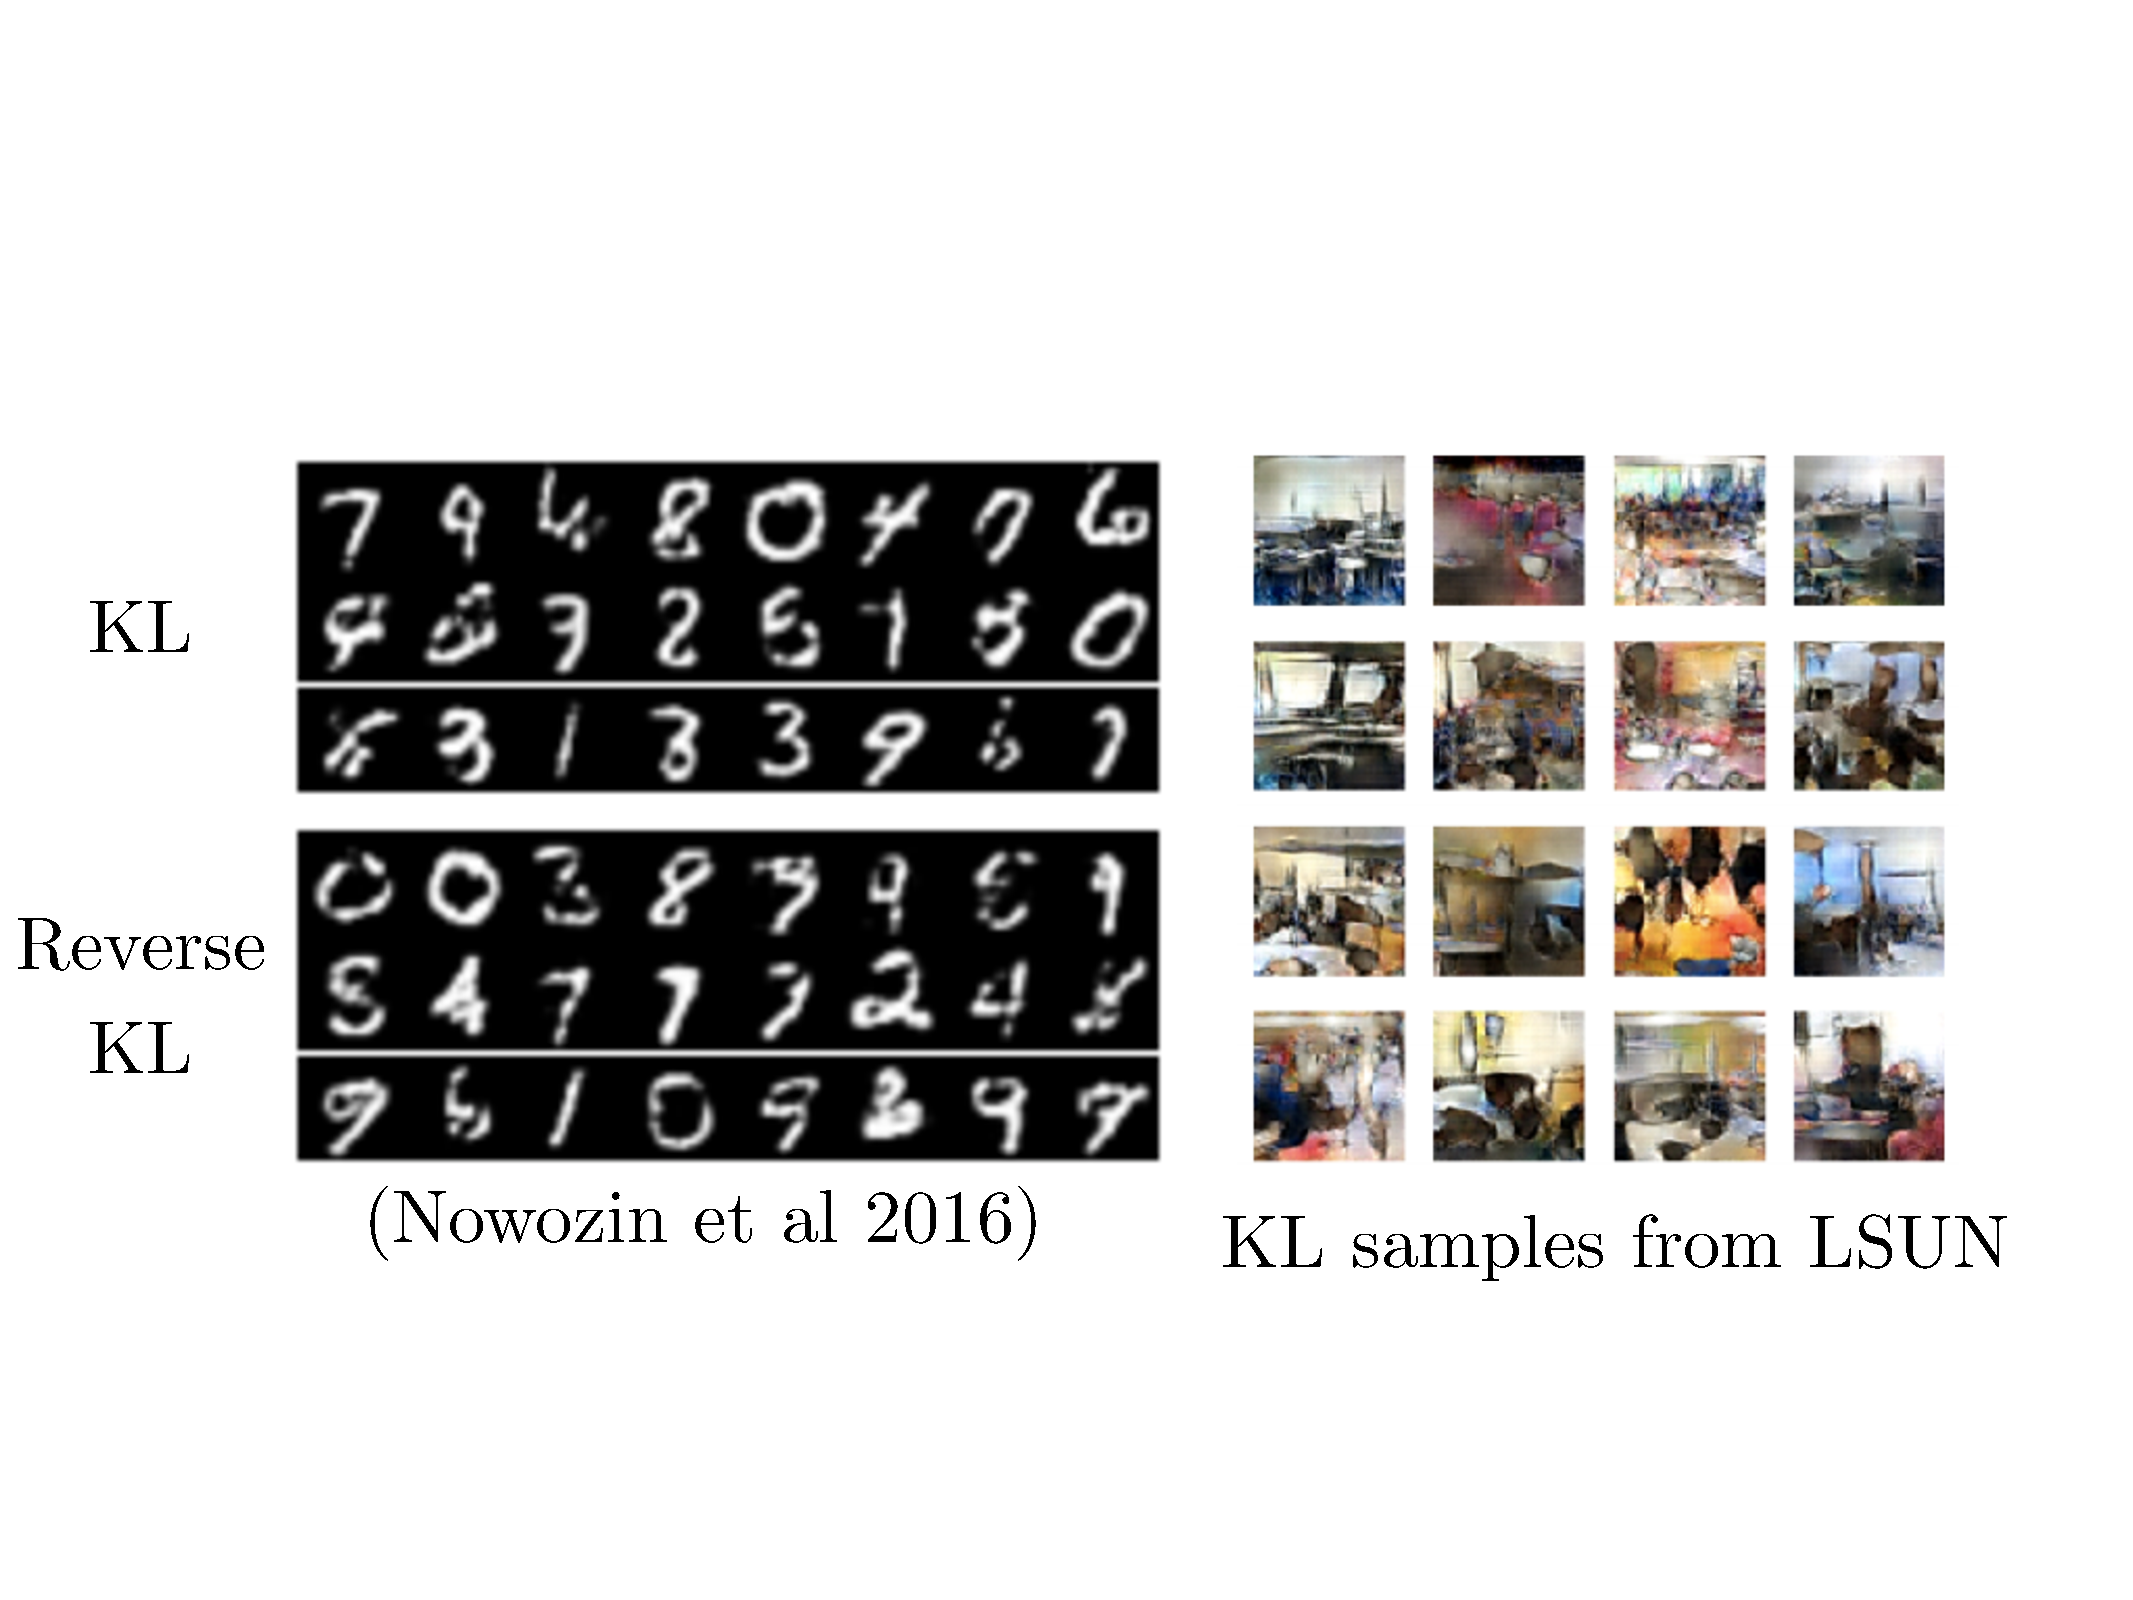
\includegraphics[width=\figwidth]{fgan}
\caption{
The f-GAN model is able to minimize many different divergences.
Because models trained to minimize $\KL(\pdata \Vert \pmodel)$
still generate sharp samples and tend to select a small number
of modes, we can conclude that the use of the Jensen-Shannon
divergence is not a particular important distinguishing
characteristic of GANs and that it does not explain why their
samples tend to be sharp.
}
\label{fig:fgan}
\end{figure}

Altogether, this suggests that GANs choose to generate a small number of modes
due to a defect in the training procedure, rather than due to the divergence
they aim to minimize.
This is discussed further in \secref{sec:mode_collapse}.
The reason that GANs produce sharp samples is not entirely clear.
It may be that the family of models trained using GANs is different from the family
of models trained using VAEs (for example, with GANs it is easy to make models
where $\vx$ has a more complicated distribution than just an isotropic Gaussian
conditioned on the input to the generator).
It may also be that the kind of approximations that GANs make have different
effects than the kind of approximations that other frameworks make.

\subsubsection{Comparison of cost functions}

We can think of the generator network as learning by a strange kind of reinforcement
learning.
Rather than being told a specific output $\vx$ it should associate with each $\vz$,
the generator takes actions and receives rewards for them.
In particular, note that $J^{(G)}$ does not make reference to the training data
directly at all; all information about the training data comes only through what
the discriminator has learned. (Incidentally, this makes GANs resistant to overfitting,
because the generator has no opportunity in practice to directly copy training examples)
The learning process differs somewhat from traditional reinforcement learning because
\begin{itemize}
 \item The generator is able to observe not just the output of the reward function but
   also its gradients.
 \item The reward function is non-stationary; the reward is based on the discriminator
   which learns in response to changes in the generator's policy.
   \end{itemize}

In all cases, we can think of the sampling process that begins with the selection of
a specific $\vz$ value as an episode that receives a single reward, independent of the
actions taken for all other $\vz$ values.
The reward given to the generator is a function of a single scalar value,
$D(G(\vz))$.
We usually think of this in terms of cost (negative reward).
The cost for the generator is always monotonically decreasing in $D(G(\vz))$ but
different games are designed to make this cost decrease faster along different parts of the curve.

\Figref{fig:comparison} shows the cost response curves as functions of $D(G(\vz))$ for three
different variants of the GAN game.
We see that the maximum likelihood game gives very high variance in the cost, with most of the
cost gradient coming from the very few samples of $\vz$ that correspond to the samples that
are most likely to be real rather than fake.
The heuristically designed non-saturating cost has lower sample variance, which may explain
why it is more successful in practice.
  This suggests that variance reduction techniques could be an important research area
  for improving the performance of GANs, especially GANs based on maximum likelihood.

\begin{figure}
\centering
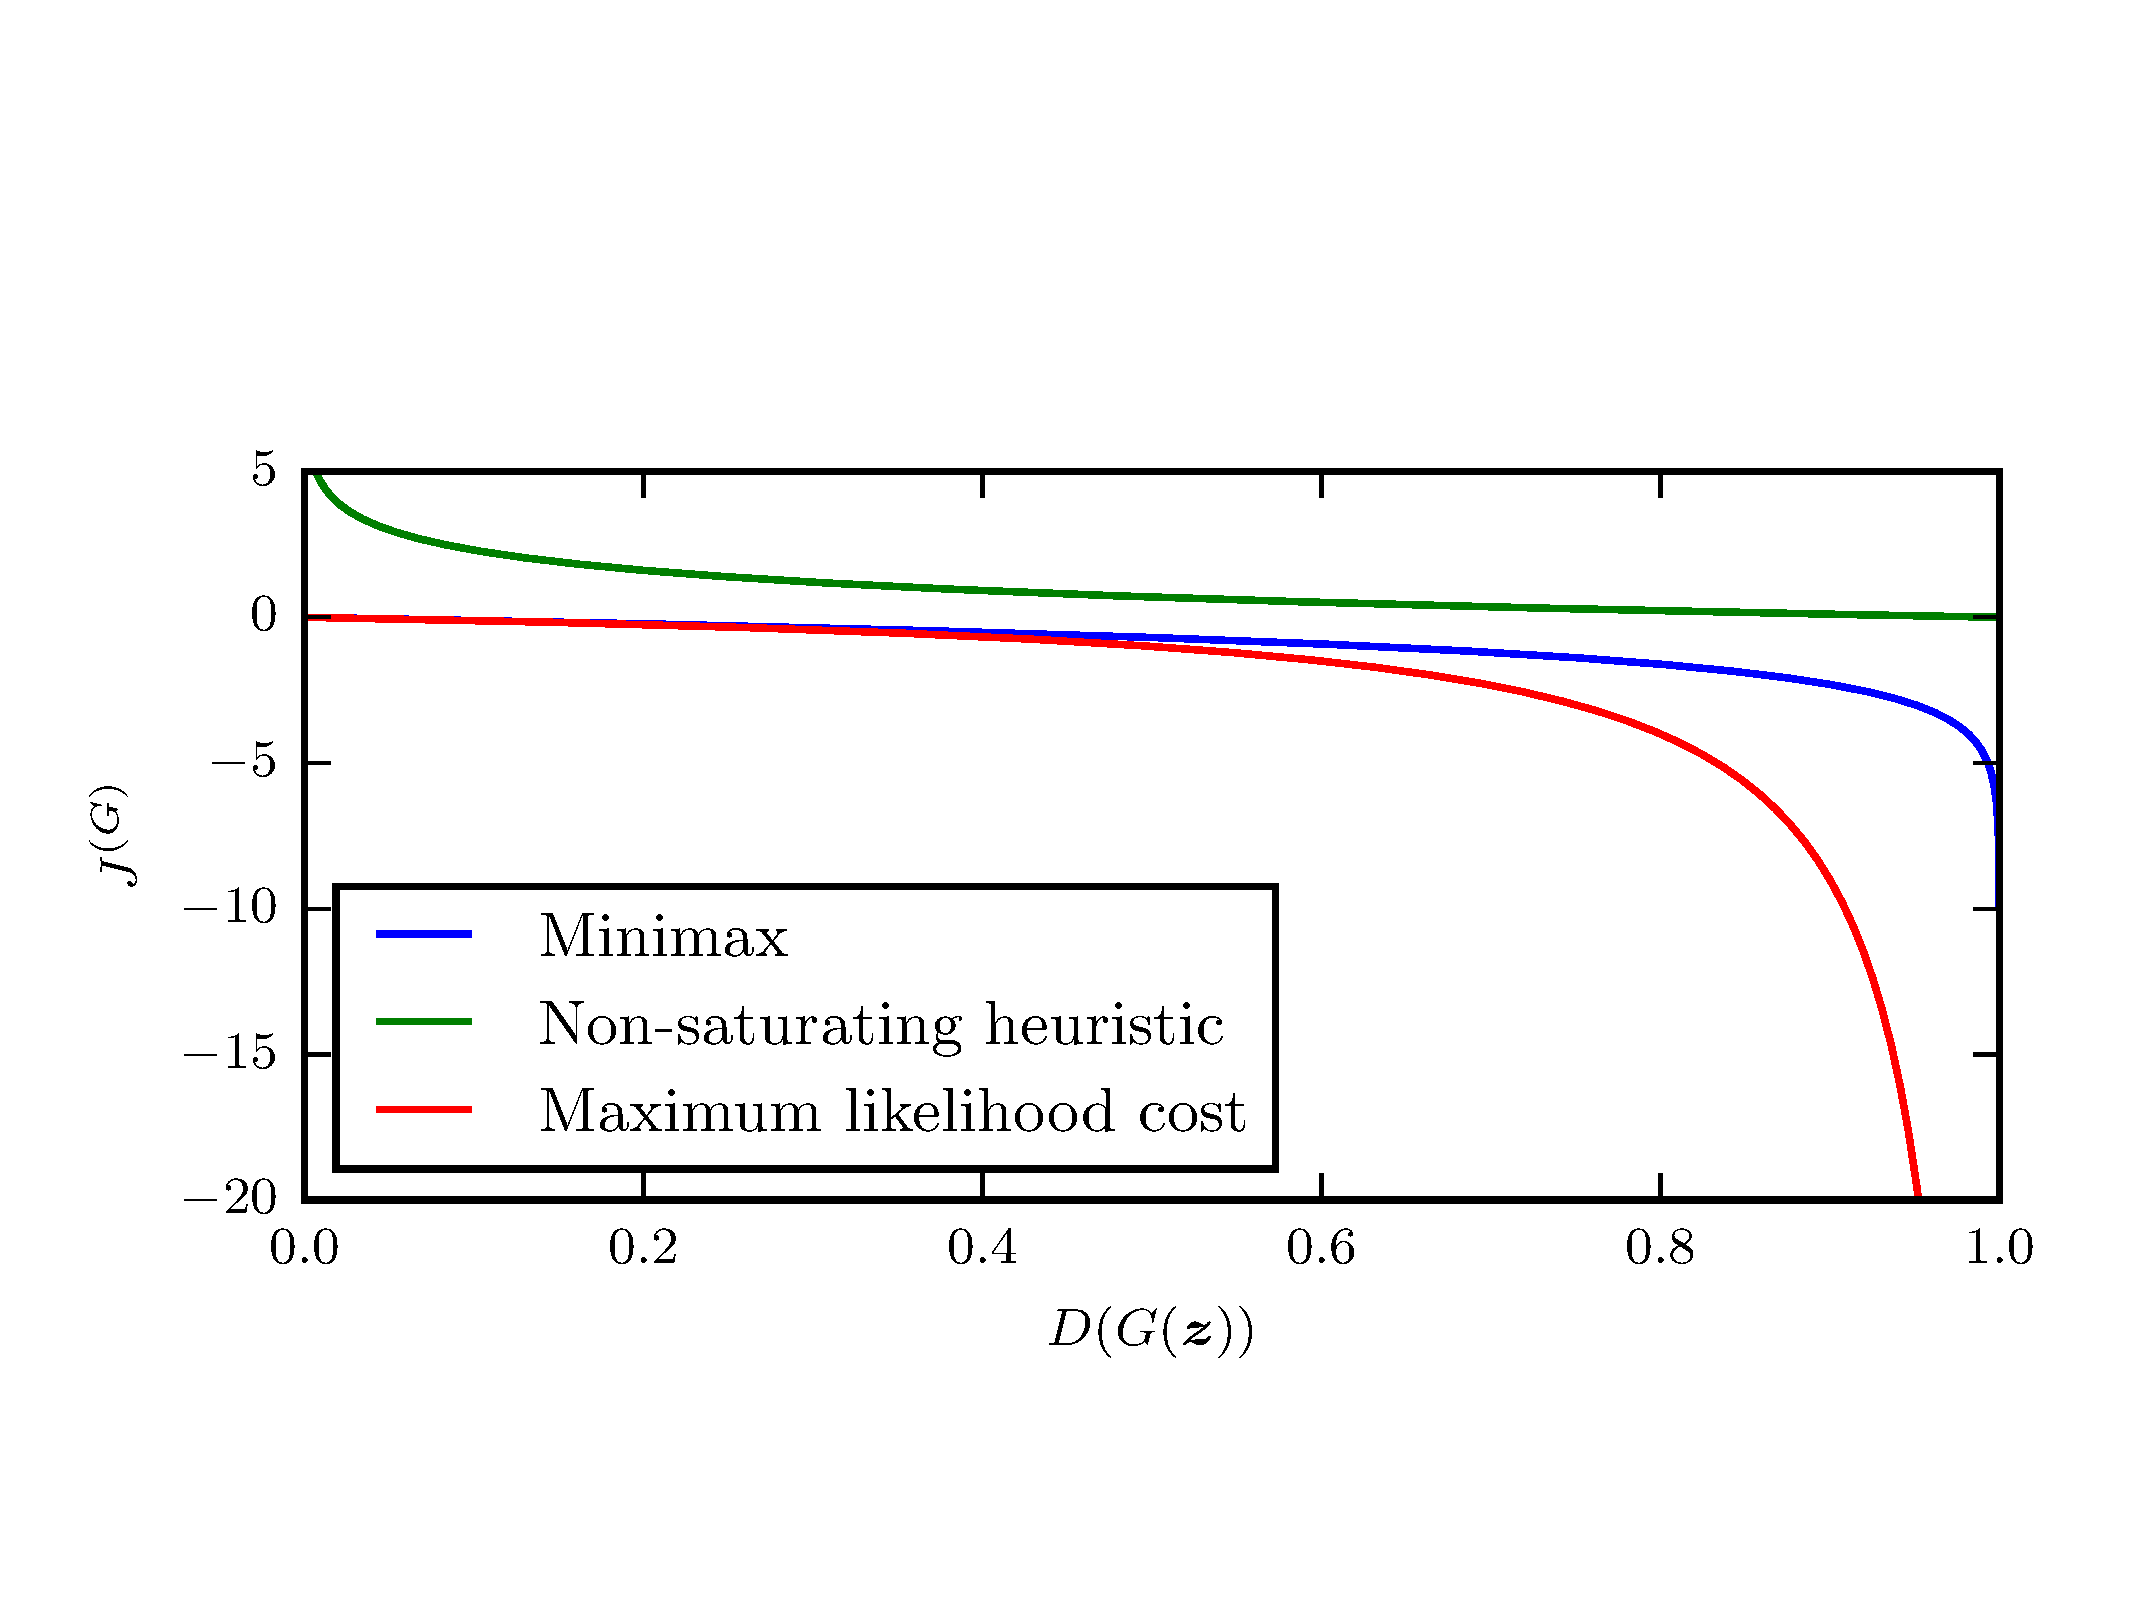
\includegraphics[width=\figwidth]{comparison}
\caption{
  The cost that the generator receives for generating a samples $G(\vz)$ depends only on
  how the discriminator responds to that sample.
  The more probability the discriminator assigns to the sample being real, the less cost
  the generator receives.
  We see that when the sample is likely to be fake, both the minimax game and the maximum
  likelihood game have very little gradient, on the flat left end of the curve.
  The heuristically motivated non-saturating cost avoids this problem.
  Maximum likelihood also suffers from the problem that nearly all of the gradient comes
  from the right end of the curve, meaning that a very small number of samples dominate
  the gradient computation for each minibatch.
  This suggests that variance reduction techniques could be an important research area
  for improving the performance of GANs, especially GANs based on maximum likelihood.
  Figure reproduced from \citet{Goodfellow-ICLR2015}.
}
\label{fig:comparison}
\end{figure}



\subsection{The DCGAN architecture}

Most GANs today are at least loosely based on the DCGAN architecture \citep{radford2015unsupervised}.
DCGAN stands for ``deep, convolution GAN.'' Though GANs were both deep and convolutional prior to
DCGANs, the name DCGAN is useful to refer to this specific style of architecture.
Some of the key insights of the DCGAN architecture were to:
\begin{itemize}
  \item Use batch normalization \citep{Ioffe+Szegedy-2015} layers in most layers of both the discriminator and the generator,
        with the two minibatches for the discriminator normalized separately.
        The last layer of the generator and first layer of the discriminator are not batch normalized,
        so that the model can learn the correct mean and scale of the data distribution.
        See \figref{fig:dcgan}.
  \item The overall network structure is mostly borrowed from the all-convolutional net \citep{Springenberg2015}.
        This architecture contains neither pooling nor ``unpooling'' layers.
        When the generator needs to increase the spatial dimension of the representation
        it uses transposed convolution with a stride greater than 1.
  \item The use of the Adam optimizer rather than SGD with momentum.
\end{itemize}

\begin{figure}
\centering
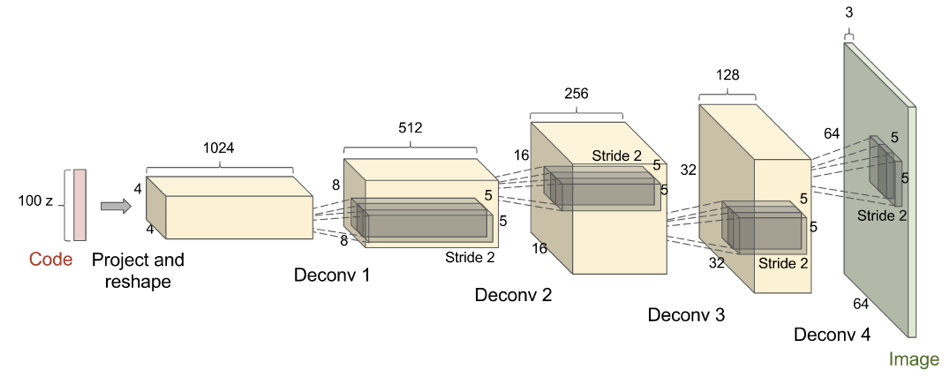
\includegraphics[width=\textwidth]{dcgan}
  \caption{The generator network used by a DCGAN. Figure reproduced from \citet{radford2015unsupervised}.}
\label{fig:dcgan}
\end{figure}

Prior to DCGANs, LAPGANs \citep{denton2015deep} were the only version of GAN
that had been able to scale to high resolution images.
LAPGANs require a multi-stage generation process in which multiple GANs
generate different levels of detail in a Laplacian pyramid representation
of an image.
DCGANs were the first GAN model to learn to generate high resolution images
in a single shot.
As shown in \figref{fig:dcgan_lsun}, DCGANs are able to generate high quality
images when trained on restricted domains of images, such as images of bedrooms.
DCGANs also clearly demonstrated that GANs learn to use their latent code
in meaningful ways, with simple arithmetic operations in latent space
having clear interpretation as arithmetic operations on semantic attributes
of the input, as demonstrated in \figref{fig:dcgan_face_arithmetic}.


\begin{figure}
  \centering
  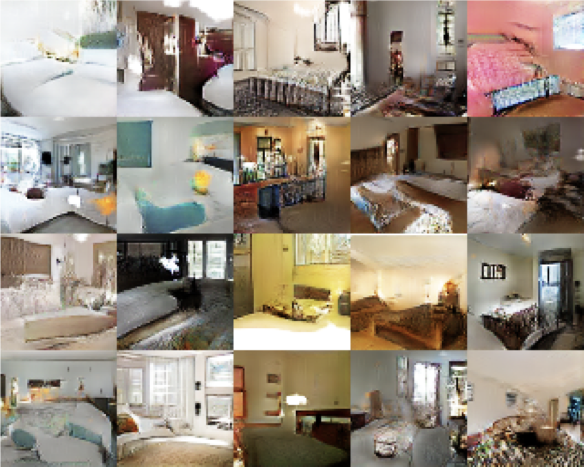
\includegraphics[width=\figwidth]{dcgan_lsun}
  \caption{Samples of images of bedrooms generated by a DCGAN trained on the LSUN dataset.}
  \label{fig:dcgan_lsun}
\end{figure}

\begin{figure}
\centering
$
\vcenter{
    \hbox{%
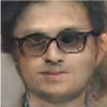
\includegraphics[width=.15\figwidth]{man_with_glasses.png} %
    }
}
\vcenter{\hbox{-}} %
\vcenter{\hbox{
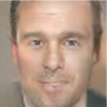
\includegraphics[width=.15\figwidth]{man_without_glasses.png} %
}}
\vcenter{\hbox{+}} %
\vcenter{\hbox{
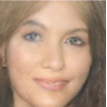
\includegraphics[width=.15\figwidth]{woman_without_glasses.png} %
}}
\vcenter{\hbox{=}} %
\vcenter{\hbox{
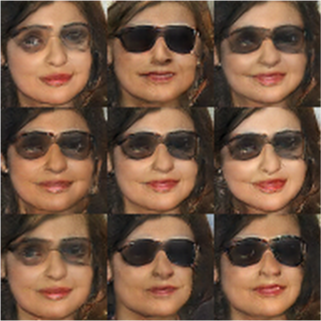
\includegraphics[width=.45\figwidth]{woman_with_glasses.png}
}
}
$
\caption{DCGANs demonstrated that GANs can learn a distributed representation
that disentangles the concept of gender from the concept of wearing
glasses. If we begin with the representation of the concept of a
man with glasses, then subtract the vector representing the concept
of a man without glasses, and finally add the vector representing
the concept of a woman without glasses, we obtain the vector representing
the concept of a woman with glasses. The generative model correctly
decodes all of these representation vectors to images that may be
recognized as belonging to the correct class.
Images reproduced from \citet{radford2015unsupervised}.
}
\label{fig:dcgan_face_arithmetic}
\end{figure}

\subsection{How do GANs relate to noise-contrastive estimation and maximum likelihood?}

While trying to understand how GANs work, one might naturally wonder about
how they are connected to \newterm{noise-constrastive estimation} (NCE)
\citep{Gutmann+Hyvarinen-2010}.
Minimax GANs use the cost function from NCE as their value function, so the
methods seem closely related at face value.
It turns out that they actually learn very different things, because the
two methods focus on different players within this game.
Roughly speaking, the goal of NCE is to learn the density model within the
discriminator, while the goal of GANs is to learn the sampler defining
the generator.
While these two tasks seem closely related at a qualitative level, the
gradients for the tasks are actually quite different.
Surprisingly, maximum likelihood turns out to be closely related to NCE,
and corresponds to playing a minimax game with the same value function,
but using a sort of heuristic update strategy rather than gradient descent
for one of the two players.
The connections are summarized in \figref{fig:nce}.

\begin{figure}
\centering
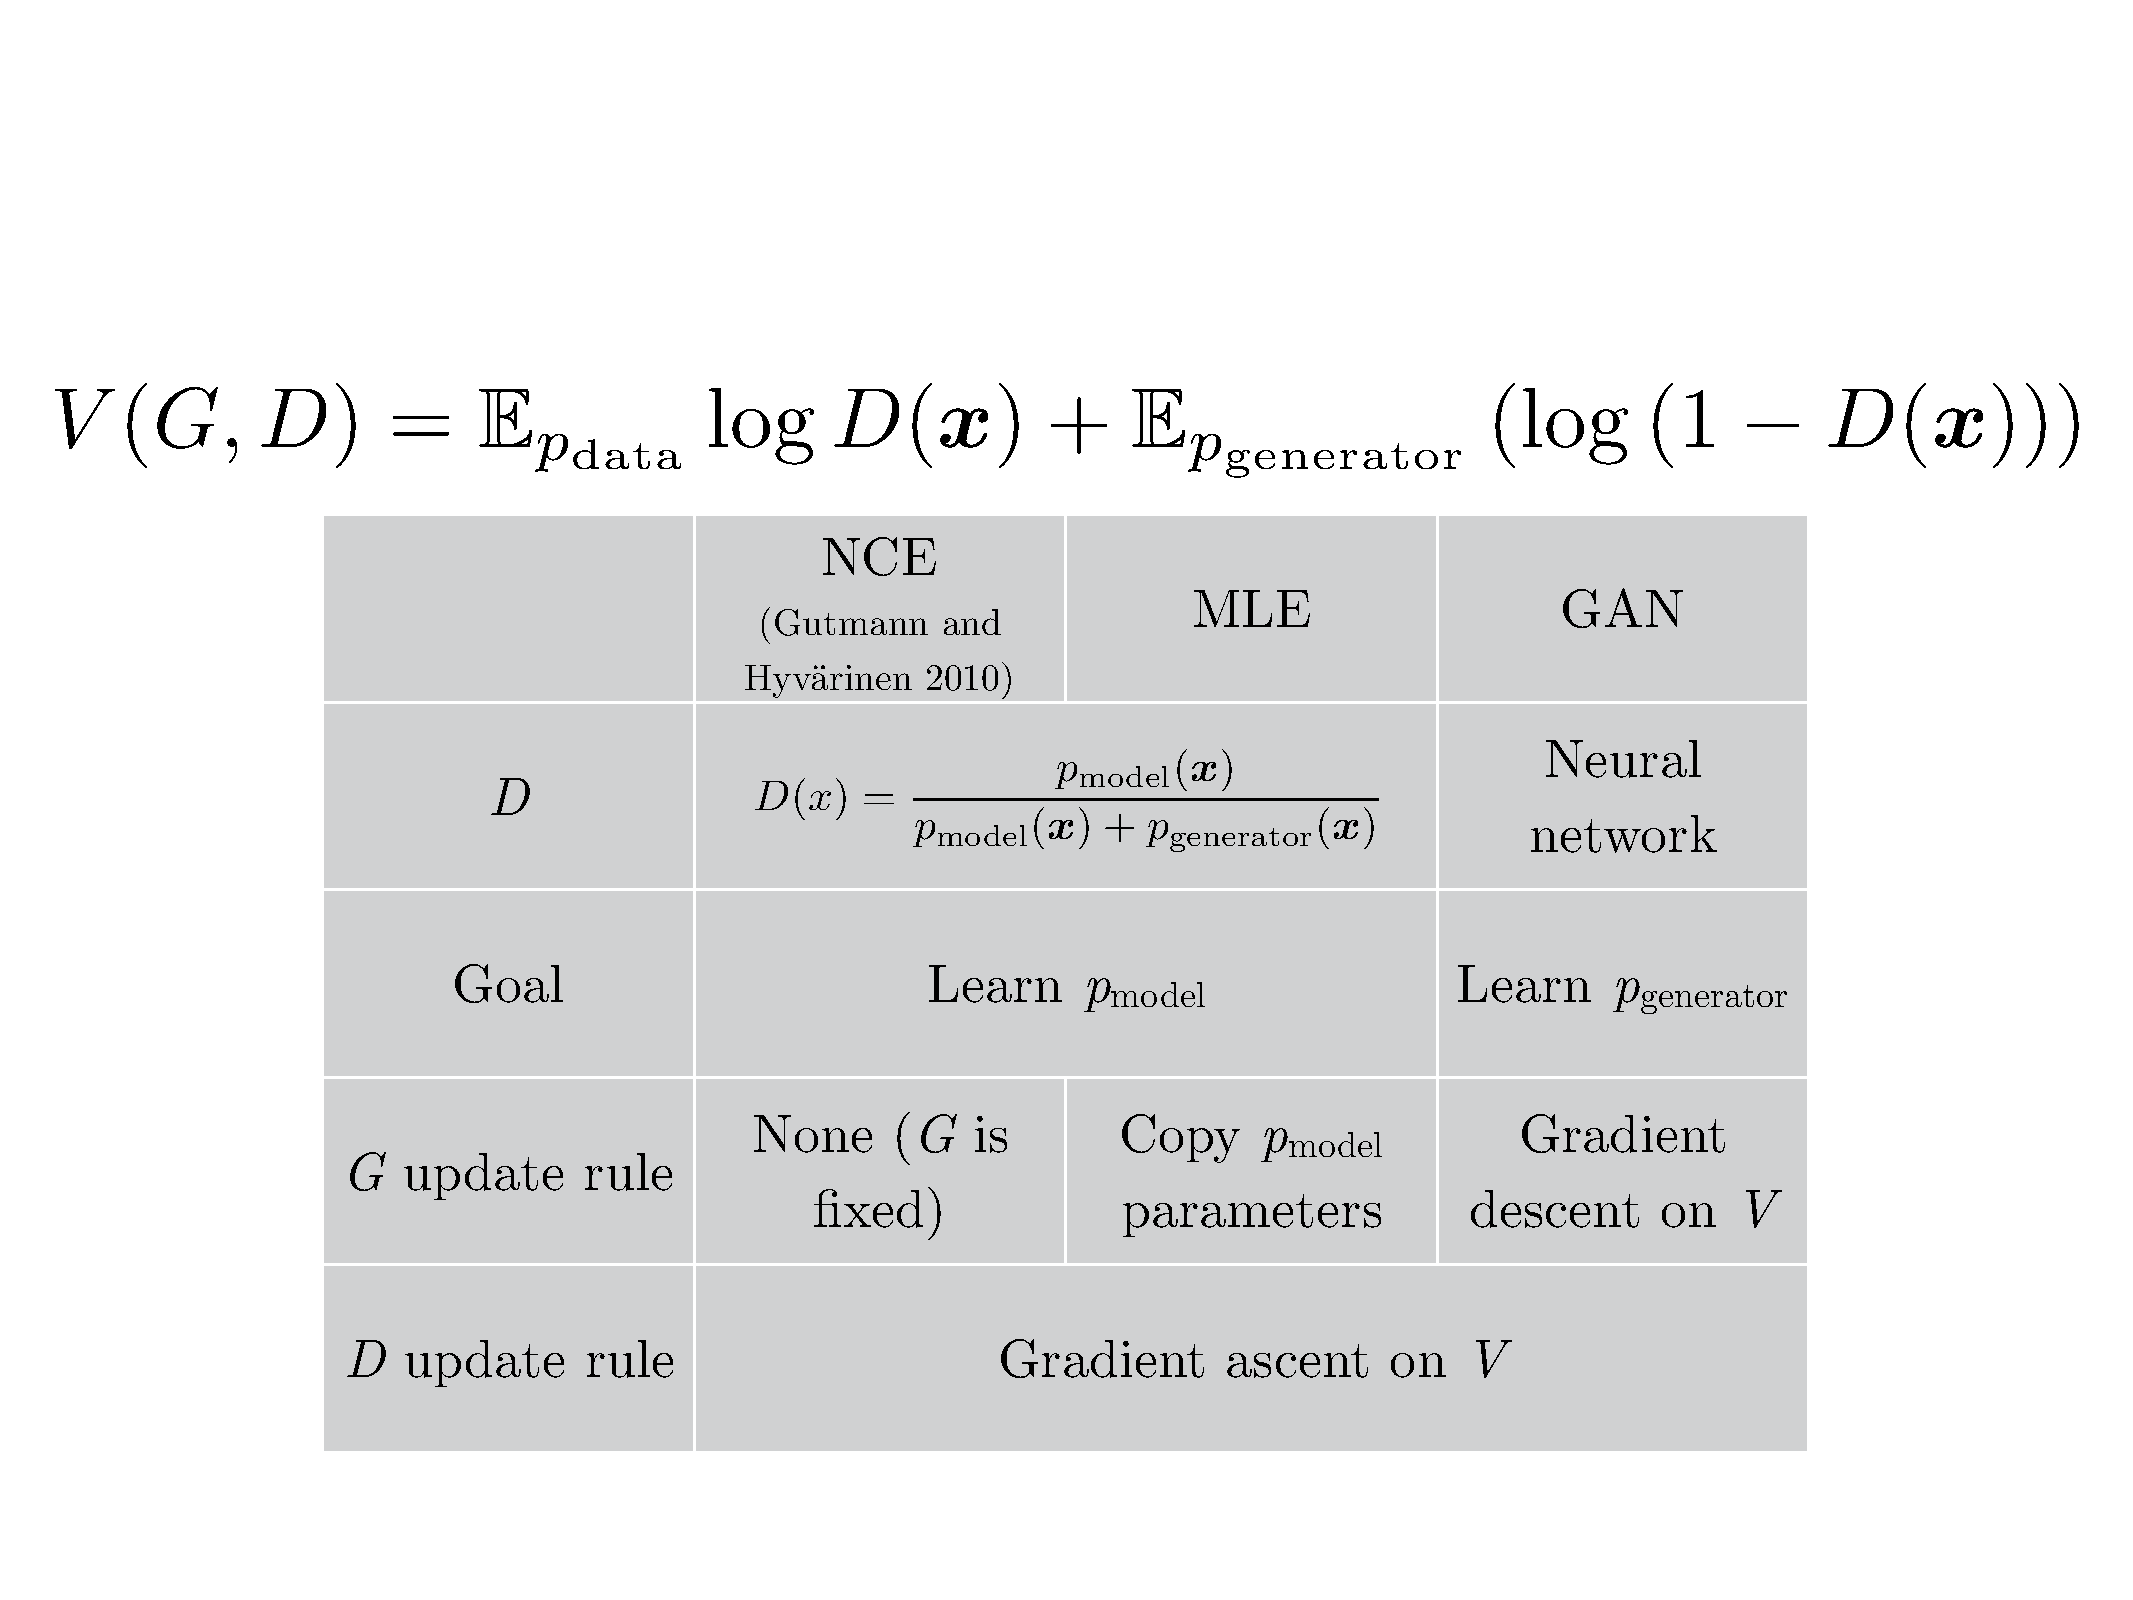
\includegraphics[width=\figwidth]{nce}
\caption{
  \citet{Goodfellow-ICLR2015} demonstrated the following
  connections between minimax GANs, noise-contrastive estimation, and
  maximum likelihood: all three can be interpreted as strategies
  for playing a minimax game with the same value function.
  The biggest difference is in where $\pmodel$ lies.
  For GANs, the generator is $\pmodel$, while for NCE and MLE,
  $\pmodel$ is part of the discriminator.
  Beyond this, the differences between the methods lie in the update
  strategy.
  GANs learn both players with gradient descent.
  MLE learns the discriminator using gradient descent, but has a heuristic
  update rule for the generator.
  Specifically, after each discriminator update step, MLE copies the density model learned inside the discriminator and 
  converts it into a sampler to be used as the generator.
  NCE never updates the generator; it is just a fixed source of noise.
}
\label{fig:nce}
\end{figure}
